% --------------------------------------------------------------------------
% LaTeX embedding template for ACL/EMNLP/NeurIPS/ICLR.
%
% Drop these snippets into main.tex.  Captions live in figs/captions.tex
% (% Bold-takeaway captions for each figure. \input from main.tex.
% Each caption is a single \newcommand{\capfigN}{...}; usage:
%   \begin{figure}[t]
%     \includegraphics[width=\linewidth]{figs/fig2}
%     \caption{\capfigtwo}
%     \label{fig:depth-profile}
%   \end{figure}

\newcommand{\capfigzero}{%
\textbf{The four value-path constructions compared in this paper.}
\textbf{(a)} The true value $V^{\mathrm{real}}_l(t) = W_V \cdot \mathrm{LN}_l(h_{l-1,t})$
uses the fully contextualized hidden state.
\textbf{(b)} The embedding-projected token table $A0$ replaces the contextualized
input with the raw token embedding, isolating any value contribution that depends
on context.
\textbf{(c)} The fitted token mean $A1 = \mu_l[x_t]$ is an empirical per-layer
per-token average $V$, used as a diagnostic anchor (vocab $\times d$ per layer;
not deployable as-is).
\textbf{(d)} Our deployable correction adds a closed-form ridge readout of
$\mathrm{LN}_l(h)$ onto $A1$, capturing the post-anchor context residual without
SGD training. The four are isolated in our forward-hook intervention;
\S\ref{sec:results} quantifies each.}

\newcommand{\capfigone}{%
\textbf{Replacing $V$ with a token-determined anchor is cheap mid-stack,
expensive at the boundaries.}
Per-layer NLL increase $\Delta$ when the V-projection at layer $l$ is
swapped for the A0 (embed-projected) anchor. The cost concentrates at
embedding-near and head-near layers; a wide mid-stack band is nearly free.
Pythia-410M, eval split (1k sequences).}

\newcommand{\capfigtwo}{%
\textbf{Most layer-wise value-ablation cost is token-determined; genuine
contextualization concentrates mid-stack, and the profile replicates across
scale.} Top: Pythia-410M (24 layers). Bottom: Pythia-160M (12 layers). Left
column: $R_{\mathrm{total}}$ under the A1 anchor is U-shaped over depth with
a sharp trough (410M: L6/L7; 160M: L4/L5). Right column: each layer's
v0 ablation cost split into A1-recoverable (blue) and residual context
(red). Trough layers are the only layers where a context signal beyond the
token is required.}

\newcommand{\capfigthree}{%
\textbf{Both A0 and A1 are context-free per-token values, yet A0 recovers
$\approx 0$ and A1 recovers $0.59$--$0.87$ -- most of the v0 ablation cost
is a weak token anchor, not contextualization.}
Recovery vs. depth on Pythia-410M. Oracle PCA of the residual at rank 256
(green) is high everywhere. The A1 trough at L6/L7 (circled) marks the
context-bound region.}

\newcommand{\capfigfour}{%
\textbf{The residual $V - A_1$ is low-rank near the boundary but
high-effective-rank in the trough.}
Eigenvalue spectrum of the per-layer residual covariance at L5 (easy) and
L11 (trough). L5 collapses to a few directions; L11 spreads mass over
$>50$ directions. The trough is not architectural incompressibility but a
linearly recoverable, broad-band context signal.}

\newcommand{\capfigfive}{%
\textbf{SGD on the trough layer L11 stalls -- not because the residual is
intrinsically hard, but because the loss surface is pathological.}
Left: training-loss trajectories under matched LR/steps/batch for several
ranks. Right: closed-form ridge solution at the same ranks. Ridge reaches
the loss SGD cannot, in one shot.}

\newcommand{\capfigsix}{%
\textbf{Closed-form ridge wins across ranks.}
Test $R_{\mathrm{context}}$ vs. rank at L11. SGD plateau (gray band) is
crossed by ridge at every rank tested; the gap widens with rank.}

\newcommand{\capfigseven}{%
\textbf{Ridge recovers the context residual at every depth.}
Left: ridge $R_{\mathrm{context}}$ vs. layer at $r=64$. Right: ridge minus
A1 baseline, per layer. The trough layers (L6/L7) are where ridge adds
the most, but the win is positive everywhere.}

\newcommand{\capfigeight}{%
\textbf{Closed-form ridge matches or beats matched-step SGD finetune.}
Per-layer test loss for ridge (closed-form) vs. SGD-finetuned LoRA at
matched ranks. The ridge bar equals or exceeds the SGD bar at every layer;
the SGD-loss surface is the bottleneck, not the corrector capacity.}

\newcommand{\capfignine}{%
\textbf{Ridge calibration scales gracefully with corpus size.}
$R_{\mathrm{context}}$ at L7 as a function of the number of calibration
tokens. The curve flattens by $\sim 4$M tokens, indicating that A1 + ridge
is data-cheap to deploy.}
 in your preamble).
% --------------------------------------------------------------------------

% --- Preamble ---
% \usepackage{graphicx}
% \usepackage{caption}
% \captionsetup{font=small,labelfont=bf,skip=4pt}
% \graphicspath{{figs/}}
% % Bold-takeaway captions for each figure. \input from main.tex.
% Each caption is a single \newcommand{\capfigN}{...}; usage:
%   \begin{figure}[t]
%     \includegraphics[width=\linewidth]{figs/fig2}
%     \caption{\capfigtwo}
%     \label{fig:depth-profile}
%   \end{figure}

\newcommand{\capfigzero}{%
\textbf{The four value-path constructions compared in this paper.}
\textbf{(a)} The true value $V^{\mathrm{real}}_l(t) = W_V \cdot \mathrm{LN}_l(h_{l-1,t})$
uses the fully contextualized hidden state.
\textbf{(b)} The embedding-projected token table $A0$ replaces the contextualized
input with the raw token embedding, isolating any value contribution that depends
on context.
\textbf{(c)} The fitted token mean $A1 = \mu_l[x_t]$ is an empirical per-layer
per-token average $V$, used as a diagnostic anchor (vocab $\times d$ per layer;
not deployable as-is).
\textbf{(d)} Our deployable correction adds a closed-form ridge readout of
$\mathrm{LN}_l(h)$ onto $A1$, capturing the post-anchor context residual without
SGD training. The four are isolated in our forward-hook intervention;
\S\ref{sec:results} quantifies each.}

\newcommand{\capfigone}{%
\textbf{Replacing $V$ with a token-determined anchor is cheap mid-stack,
expensive at the boundaries.}
Per-layer NLL increase $\Delta$ when the V-projection at layer $l$ is
swapped for the A0 (embed-projected) anchor. The cost concentrates at
embedding-near and head-near layers; a wide mid-stack band is nearly free.
Pythia-410M, eval split (1k sequences).}

\newcommand{\capfigtwo}{%
\textbf{Most layer-wise value-ablation cost is token-determined; genuine
contextualization concentrates mid-stack, and the profile replicates across
scale.} Top: Pythia-410M (24 layers). Bottom: Pythia-160M (12 layers). Left
column: $R_{\mathrm{total}}$ under the A1 anchor is U-shaped over depth with
a sharp trough (410M: L6/L7; 160M: L4/L5). Right column: each layer's
v0 ablation cost split into A1-recoverable (blue) and residual context
(red). Trough layers are the only layers where a context signal beyond the
token is required.}

\newcommand{\capfigthree}{%
\textbf{Both A0 and A1 are context-free per-token values, yet A0 recovers
$\approx 0$ and A1 recovers $0.59$--$0.87$ -- most of the v0 ablation cost
is a weak token anchor, not contextualization.}
Recovery vs. depth on Pythia-410M. Oracle PCA of the residual at rank 256
(green) is high everywhere. The A1 trough at L6/L7 (circled) marks the
context-bound region.}

\newcommand{\capfigfour}{%
\textbf{The residual $V - A_1$ is low-rank near the boundary but
high-effective-rank in the trough.}
Eigenvalue spectrum of the per-layer residual covariance at L5 (easy) and
L11 (trough). L5 collapses to a few directions; L11 spreads mass over
$>50$ directions. The trough is not architectural incompressibility but a
linearly recoverable, broad-band context signal.}

\newcommand{\capfigfive}{%
\textbf{SGD on the trough layer L11 stalls -- not because the residual is
intrinsically hard, but because the loss surface is pathological.}
Left: training-loss trajectories under matched LR/steps/batch for several
ranks. Right: closed-form ridge solution at the same ranks. Ridge reaches
the loss SGD cannot, in one shot.}

\newcommand{\capfigsix}{%
\textbf{Closed-form ridge wins across ranks.}
Test $R_{\mathrm{context}}$ vs. rank at L11. SGD plateau (gray band) is
crossed by ridge at every rank tested; the gap widens with rank.}

\newcommand{\capfigseven}{%
\textbf{Ridge recovers the context residual at every depth.}
Left: ridge $R_{\mathrm{context}}$ vs. layer at $r=64$. Right: ridge minus
A1 baseline, per layer. The trough layers (L6/L7) are where ridge adds
the most, but the win is positive everywhere.}

\newcommand{\capfigeight}{%
\textbf{Closed-form ridge matches or beats matched-step SGD finetune.}
Per-layer test loss for ridge (closed-form) vs. SGD-finetuned LoRA at
matched ranks. The ridge bar equals or exceeds the SGD bar at every layer;
the SGD-loss surface is the bottleneck, not the corrector capacity.}

\newcommand{\capfignine}{%
\textbf{Ridge calibration scales gracefully with corpus size.}
$R_{\mathrm{context}}$ at L7 as a function of the number of calibration
tokens. The curve flattens by $\sim 4$M tokens, indicating that A1 + ridge
is data-cheap to deploy.}


% --------------------------------------------------------------------------
% Fig 0: schematic. PRIMARY source is figs/fig0_schematic.tex (TikZ,
% hand-drawn 4-panel V-derivation pipeline). Two usage modes:
%
% Mode 1 (standalone-compile, recommended): compile fig0_schematic.tex with
%   pdflatex to produce fig0.pdf, then include like the other figures:
%     \begin{figure}[t]
%       \centering
%       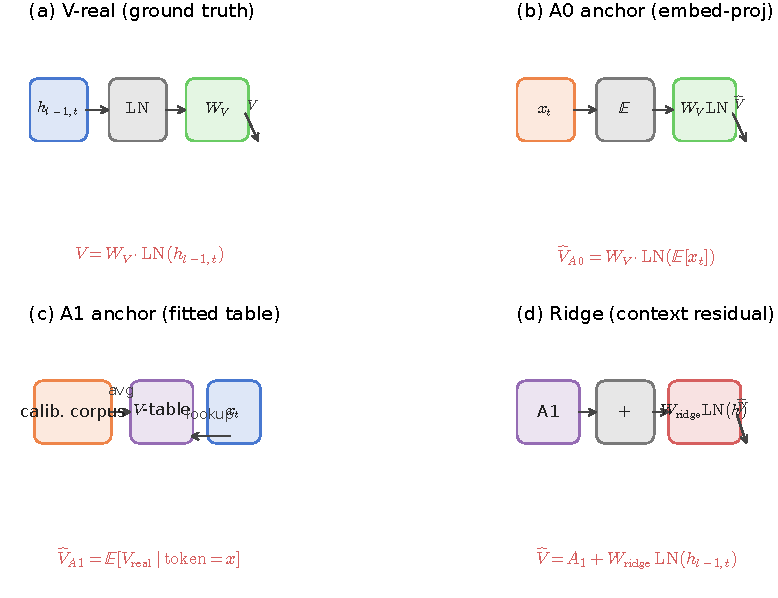
\includegraphics[width=\linewidth]{fig0.pdf}
%       \caption{\capfigzero}
%       \label{fig:schematic}
%     \end{figure}
%
% Mode 2 (inline): copy the \tikzset block from fig0_schematic.tex into the
%   main.tex preamble, then drop the \begin{tikzpicture}...\end{tikzpicture}
%   block inside a figure environment:
%     \begin{figure}[t]
%       \centering
%       \begin{tikzpicture}[panel sep/.style={node distance=2.0mm and 3.5mm},
%                           inner sep=0pt, outer sep=0pt]
%         % ...  body from Version A of fig0_schematic.tex  ...
%       \end{tikzpicture}
%       \caption{\capfigzero}
%       \label{fig:schematic}
%     \end{figure}
%
% Fallback (no LaTeX runtime): include the matplotlib-rendered fig0.pdf
% produced by fig0_schematic.py.  Same \includegraphics line as Mode 1.
% --------------------------------------------------------------------------
\begin{figure}[t]
  \centering
  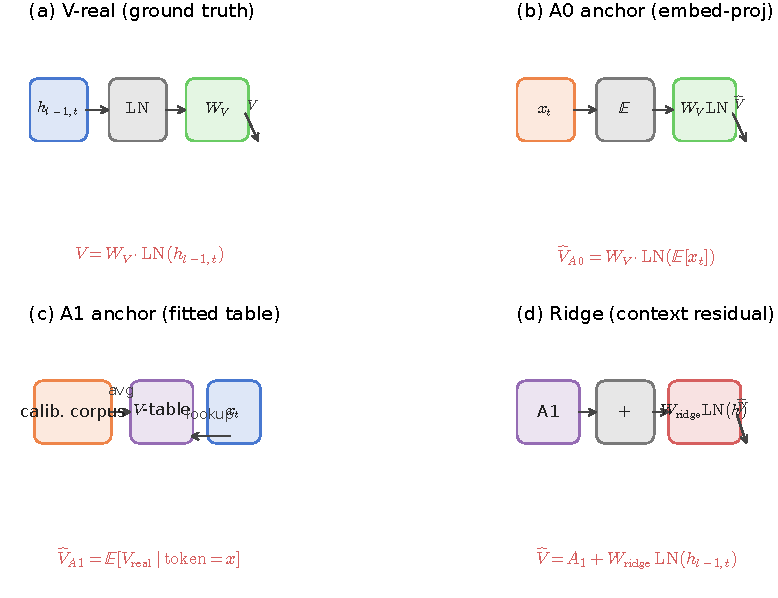
\includegraphics[width=\linewidth]{fig0.pdf}
  \caption{\capfigzero}
  \label{fig:schematic}
\end{figure}

% --------------------------------------------------------------------------
% Fig 1: single column.
% --------------------------------------------------------------------------
\begin{figure}[t]
  \centering
  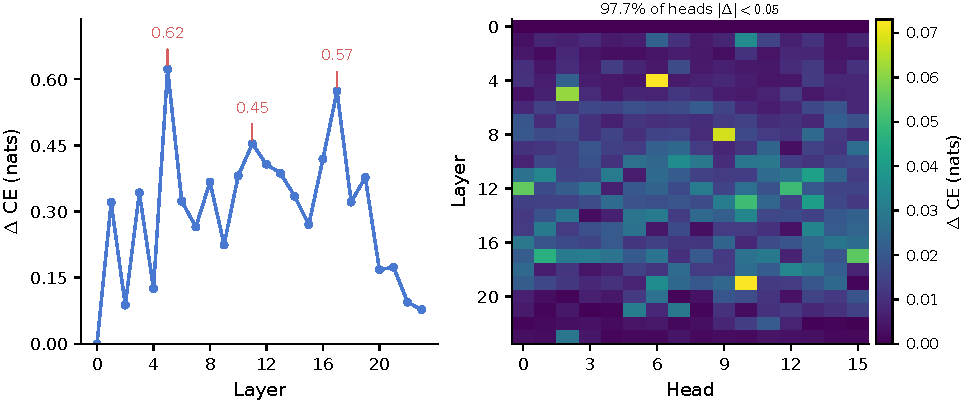
\includegraphics[width=\linewidth]{fig1.pdf}
  \caption{\capfigone}
  \label{fig:v0-heatmap}
\end{figure}

% --------------------------------------------------------------------------
% Fig 2: double-column 2x2 (cross-scale depth profile).  Use figure* in
% two-column templates (ACL, NeurIPS).
% --------------------------------------------------------------------------
\begin{figure*}[t]
  \centering
  \includegraphics[width=\textwidth]{fig2.pdf}
  \caption{\capfigtwo}
  \label{fig:depth-profile}
\end{figure*}

% --------------------------------------------------------------------------
% Fig 3: single column.
% --------------------------------------------------------------------------
\begin{figure}[t]
  \centering
  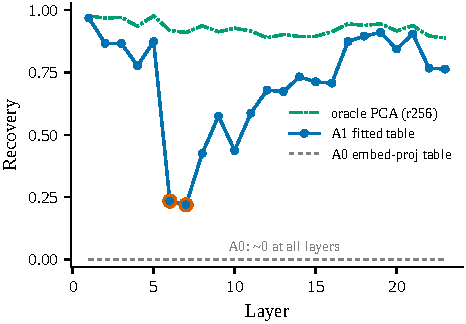
\includegraphics[width=\linewidth]{fig3.pdf}
  \caption{\capfigthree}
  \label{fig:anchor-audit}
\end{figure}

% --------------------------------------------------------------------------
% Fig 4: single column.
% --------------------------------------------------------------------------
\begin{figure}[t]
  \centering
  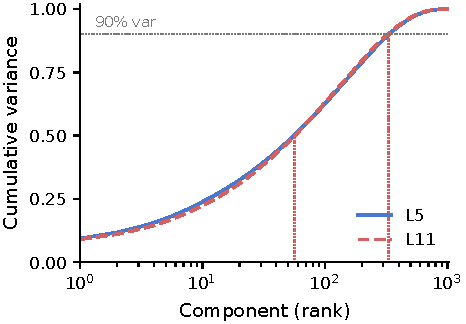
\includegraphics[width=\linewidth]{fig4.pdf}
  \caption{\capfigfour}
  \label{fig:diff-spectrum}
\end{figure}

% --------------------------------------------------------------------------
% Fig 5: double-column 2-panel.
% --------------------------------------------------------------------------
\begin{figure*}[t]
  \centering
  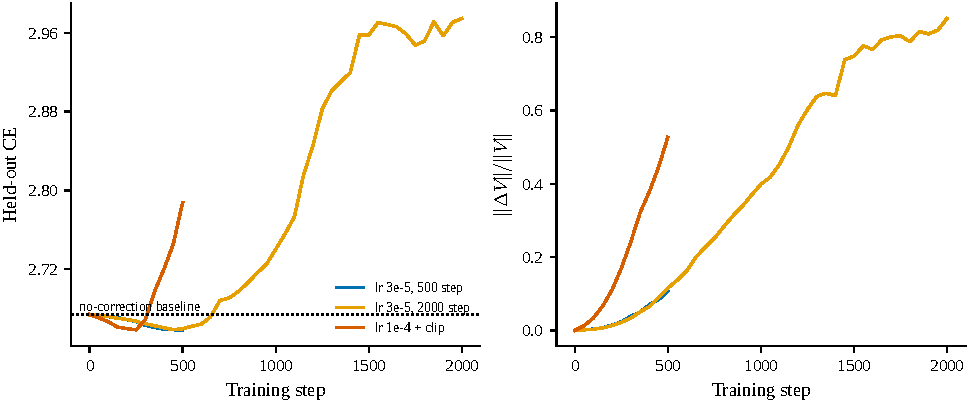
\includegraphics[width=\textwidth]{fig5.pdf}
  \caption{\capfigfive}
  \label{fig:sgd-diverges}
\end{figure*}

% --------------------------------------------------------------------------
% Fig 6: single column.
% --------------------------------------------------------------------------
\begin{figure}[t]
  \centering
  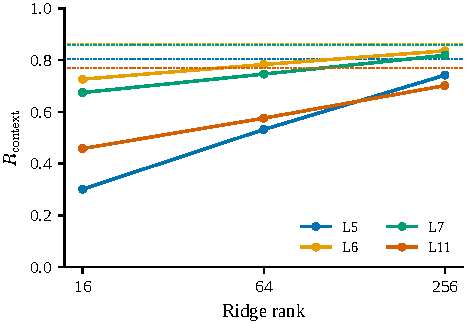
\includegraphics[width=\linewidth]{fig6.pdf}
  \caption{\capfigsix}
  \label{fig:ridge-rank}
\end{figure}

% --------------------------------------------------------------------------
% Fig 7: double-column 2-panel.
% --------------------------------------------------------------------------
\begin{figure*}[t]
  \centering
  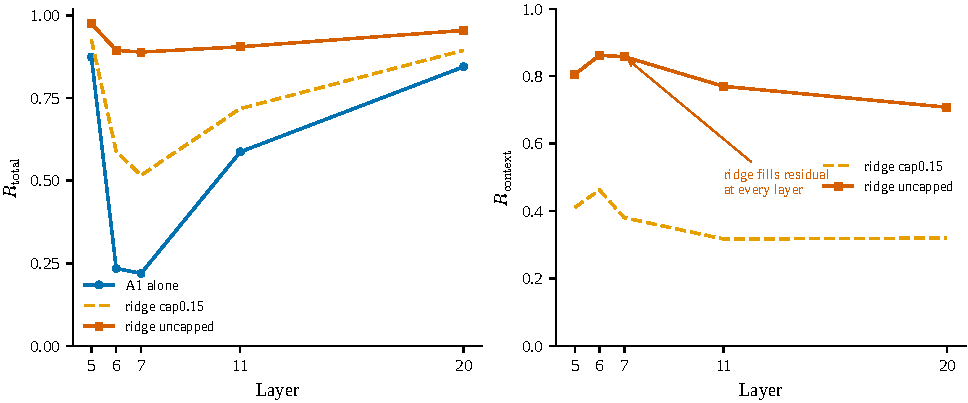
\includegraphics[width=\textwidth]{fig7.pdf}
  \caption{\capfigseven}
  \label{fig:ridge-depth}
\end{figure*}

% --------------------------------------------------------------------------
% Fig 8: single column.
% --------------------------------------------------------------------------
\begin{figure}[t]
  \centering
  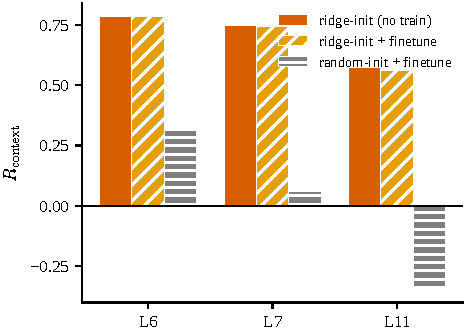
\includegraphics[width=\linewidth]{fig8.pdf}
  \caption{\capfigeight}
  \label{fig:ridge-vs-sgd}
\end{figure}

% --------------------------------------------------------------------------
% Fig 9: single column.
% --------------------------------------------------------------------------
\begin{figure}[t]
  \centering
  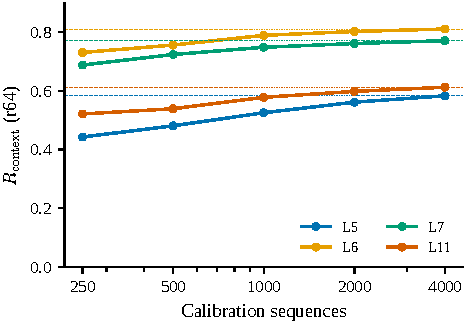
\includegraphics[width=\linewidth]{fig9.pdf}
  \caption{\capfignine}
  \label{fig:ridge-scale}
\end{figure}

% --------------------------------------------------------------------------
% Fig 11: double-column. §5.5 SGD pressure test.
% --------------------------------------------------------------------------
\begin{figure*}[t]
  \centering
  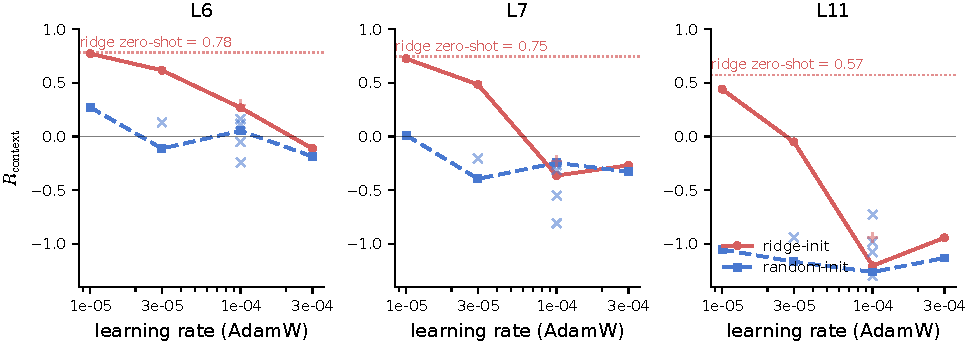
\includegraphics[width=\textwidth]{fig11.pdf}
  \caption{\capfigeleven}
  \label{fig:sgd-pressure}
\end{figure*}
